\documentclass[11pt,a4paper]{article}

\usepackage[margin=2.2cm]{geometry}
\usepackage{amsmath,amssymb,amsthm}
\usepackage{booktabs}
\usepackage{array}
\usepackage{xcolor}
\usepackage{tikz}
\usetikzlibrary{arrows.meta,positioning,fit,backgrounds,matrix,calc,shapes.geometric,decorations.pathreplacing}
\usepackage{pgfplots}
\pgfplotsset{compat=1.18}
\usepackage{algpseudocode}
\usepackage{caption}
\usepackage{float}
\usepackage{hyperref}
\hypersetup{colorlinks=true,linkcolor=blue!50!black,urlcolor=blue!50!black,citecolor=blue!50!black}

\definecolor{oldc}{RGB}{190,60,60}
\definecolor{newc}{RGB}{40,120,80}
\definecolor{varc}{RGB}{50,90,170}
\definecolor{constc}{RGB}{200,130,20}
\definecolor{paramc}{RGB}{120,60,160}
\definecolor{grey}{RGB}{120,120,120}

\newcommand{\vecF}{\operatorname{vec}_F}
\newcommand{\nnz}{\operatorname{nnz}}
\newcommand{\R}{\mathbb{R}}
\newcommand{\code}[1]{\texttt{#1}}
\newcommand{\T}{\mathsf{T}}

\title{The CVXPY Rust canonicalization backend:\\ changes of 16--17 September 2026 and why they are faster}
\author{Ray Kasichainula \and Claude (Fable 5.1)}
\date{21 September 2026}

\begin{document}
\maketitle

\begin{abstract}
Between 16 and 17 September 2026 the Rust canonicalization backend of CVXPY (branch
\code{rust-backend-pr-20260915} on \code{mellowyellow71/cvxrust}) received seven commits: a safe
availability check, three N-D correctness fixes, a rewrite of the matrix-multiplication kernels, a
rewrite of row selection and output assembly, a DAG memo for shared subexpressions, and a row
push-down for diagonal, index and trace selectors. On the five external benchmark classes that
motivated the work, cold compile time went from 9.04\,s to 0.42\,s (UnconstrainedQP), 1.29\,s to
0.38\,s (QuantumHilbertMatrix), 1.77\,s to 0.62\,s (TvInpainting), unchanged 0.35\,s (Cajas) and
from out-of-memory to 12.1\,s (SDPSegfault1132), against 5.24, 2.08, 1.03, 1.85 and 29.6\,s for the
C++ backend on the same machine. This document explains what the backend computes, what each change
does, why it is correct, and where each second went.
\end{abstract}

\tableofcontents

%======================================================================
\section{What the backend computes: matrix stuffing}
\label{sec:stuffing}

\subsection{From expressions to a coefficient tensor}

After the DCP reductions, every constraint and the objective of a problem is an affine expression of
the stacked variable vector $x \in \R^n$ and, under DPP, of the stacked parameter vector
$\theta \in \R^p$. Canonicalization (``matrix stuffing'') has to turn each such expression $f$ into
the data of a solver-ready form
\begin{equation}
  f(x;\theta) = A(\theta)\,x + b(\theta), \qquad A(\theta) \in \R^{m \times n},\ b(\theta) \in \R^{m},
\end{equation}
where $m$ is the number of scalar entries of $f$ in column-major (Fortran, ``F'') order. DPP
guarantees $A$ and $b$ are affine in $\theta$, so the whole map is a \emph{third-order tensor}
\begin{equation}
  \label{eq:tensor}
  T \in \R^{m \times (n+1) \times (p+1)}, \qquad
  [A(\theta)\ \ b(\theta)] \;=\; \sum_{k=0}^{p-1} \theta_k\, T_{:,:,k} \;+\; T_{:,:,p}.
\end{equation}
Column $n$ (the last variable column) holds the constant part $b$, and slice $p$ (the last parameter
slice) holds the part that does not depend on any parameter. Every backend
(\code{SCIPY}, \code{COO}, \code{CPP}, \code{RUST}) builds exactly this tensor; they differ only in
representation and in the order of operations.

\begin{figure}[H]
\centering
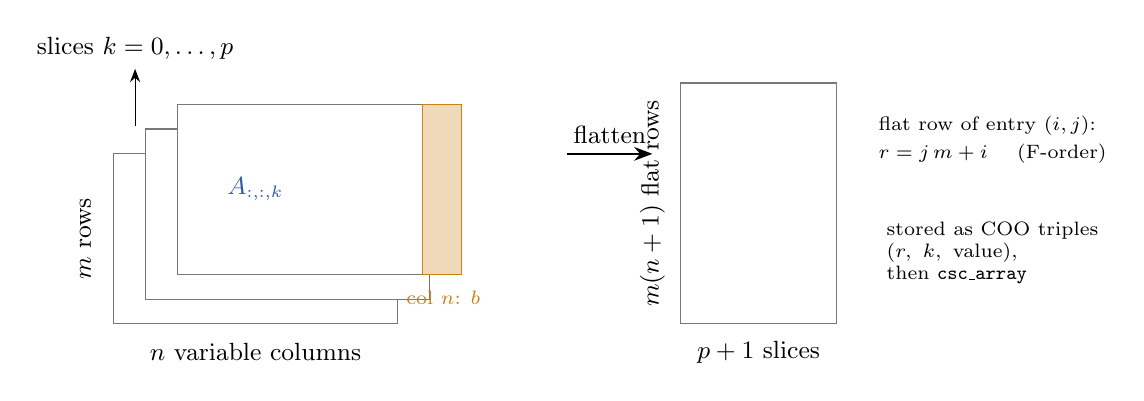
\begin{tikzpicture}[scale=0.9, every node/.style={font=\small}]
  % 3D tensor sketch
  \begin{scope}[shift={(0,0)}]
    \foreach \k/\lab in {0/{$k=p$ (constant slice)},1/{$k=1$},2/{$k=0$}} {
      \draw[fill=white, draw=grey] (0.45*\k,0.35*\k) rectangle ++(4,2.4);
    }
    \node at (2.0,-0.4) {$n$ variable columns};
    \node[rotate=90] at (-0.4,1.2) {$m$ rows};
    \draw[fill=constc!30, draw=constc] (0.9+3.45,0.7) rectangle ++(0.55,2.4);
    \node[constc, font=\scriptsize, anchor=north] at (4.65,0.6) {col $n$: $b$};
    \draw[-{Stealth}] (0.3,2.8) -- (0.3,3.6) node[above] {slices $k = 0,\dots,p$};
    \node[varc] at (2.0,1.9) {$A_{:,:,k}$};
  \end{scope}
  \draw[-{Stealth}, thick] (6.4,2.4) -- (7.6,2.4) node[midway, above] {flatten};
  % 2D flattened
  \begin{scope}[shift={(8,0)}]
    \draw[fill=white, draw=grey] (0,0) rectangle (2.2,3.4);
    \node at (1.1,-0.4) {$p+1$ slices};
    \node[rotate=90] at (-0.4,1.7) {$m(n+1)$ flat rows};
    \node[font=\scriptsize, align=left] at (4.4,2.6) {flat row of entry $(i,j)$:\\[2pt] $r = j\,m + i$ \quad (F-order)};
    \node[font=\scriptsize, align=left] at (4.4,1.0) {stored as COO triples\\ $(r,\ k,\ \text{value})$,\\ then \code{csc\_array}};
  \end{scope}
\end{tikzpicture}
\caption{The coefficient tensor \eqref{eq:tensor} and the 2-D matrix that is handed back to Python. An
entry at row $i$, variable column $j$, parameter slice $k$ becomes the COO triple $(jm+i,\,k,\,\text{value})$.}
\label{fig:tensor}
\end{figure}

\subsection{LinOp trees}

CVXPY hands each expression to the backend as a tree of \emph{LinOps}: leaves are variables,
parameters and constants; interior nodes are the linear operations (\code{neg}, \code{sum},
\code{mul} by a constant on the left, \code{rmul} by a constant on the right, \code{mul\_elem},
\code{index}, \code{transpose}, \code{vstack}, \code{diag\_mat}, \code{trace}, \code{kron\_r}, \dots).
Every node carries its shape; a variable leaf of size $s$ lowers to the identity map $I_s$ placed at
that variable's column offset, and every interior node is a linear map applied to the tensors of its
children. Lowering a tree is therefore the evaluation of a composition of linear maps on sparse
tensors, and the whole art of a backend is to keep those intermediate tensors small and the
compositions cheap.

\subsection{The Rust representation}

The Rust backend keeps every intermediate tensor in coordinate form:
\begin{equation}
  \label{eq:coo}
  \code{SparseTensor} = \big\{(\text{row}_e,\ \text{col}_e,\ \text{param}_e,\ \text{val}_e)\big\}_{e=1}^{\nnz},
\end{equation}
four parallel arrays, no ordering invariant, duplicates allowed. Duplicates mean two entries with the
same (row, col, param); their values add. The pipeline is shown in figure~\ref{fig:pipeline}. Two
properties of this design matter for everything that follows:
\begin{enumerate}
  \item An operation that maps rows to rows (negation, reshape, index, transpose, stacking, diagonal
  selection) costs $O(\nnz)$ and touches no structure.
  \item Anything that \emph{combines} entries (matrix multiplication, sums of overlapping terms) can
  only combine them by producing duplicates. Somebody has to coalesce those later, and the cost of
  coalescing is a sort of everything produced.
\end{enumerate}

\begin{figure}[H]
\centering
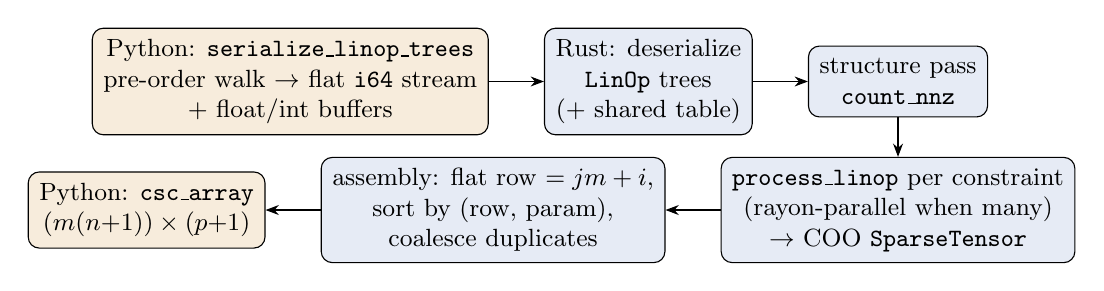
\begin{tikzpicture}[node distance=5mm and 7mm, every node/.style={font=\small},
  box/.style={draw, rounded corners, align=center, minimum height=9mm, inner sep=4pt},
  py/.style={box, fill=constc!15}, rs/.style={box, fill=varc!12}]
  \node[py] (ser) {Python: \code{serialize\_linop\_trees}\\ pre-order walk $\to$ flat \code{i64} stream\\ + float/int buffers};
  \node[rs, right=of ser] (des) {Rust: deserialize\\ \code{LinOp} trees\\ (+ shared table)};
  \node[rs, right=of des] (cnt) {structure pass\\ \code{count\_nnz}};
  \node[rs, below=of cnt] (proc) {\code{process\_linop} per constraint\\ (rayon-parallel when many)\\ $\to$ COO \code{SparseTensor}};
  \node[rs, left=of proc] (asm) {assembly: flat row $= jm+i$,\\ sort by (row, param),\\ coalesce duplicates};
  \node[py, left=of asm] (csc) {Python: \code{csc\_array}\\ $(m(n{+}1)) \times (p{+}1)$};
  \draw[-{Stealth}] (ser) -- (des);
  \draw[-{Stealth}] (des) -- (cnt);
  \draw[-{Stealth}] (cnt) -- (proc);
  \draw[-{Stealth}] (proc) -- (asm);
  \draw[-{Stealth}] (asm) -- (csc);
\end{tikzpicture}
\caption{The Rust backend pipeline. The serializer and the assembly step were both changed in this
round (sections \ref{sec:memo} and \ref{sec:assembly}); the per-node lowering is where the kernel
work of sections \ref{sec:kernel} and \ref{sec:pushdown} lives.}
\label{fig:pipeline}
\end{figure}

%======================================================================
\section{Starting point and measurements}
\label{sec:baseline}

All timings in this document are cold compile times of \code{Problem.get\_problem\_data} on one
Linux machine (single BLAS thread, one untimed warm-up, median of two, one isolated process per
class), measured with \code{rust\_benchmarks/run\_one.py} against the external benchmark classes in
\code{cvxpy/benchmarks}. The candidate branch sits on upstream \code{773163ebd}.

\begin{table}[H]
\centering
\footnotesize
\setlength{\tabcolsep}{4pt}
\resizebox{\textwidth}{!}{%
\begin{tabular}{lrrrrl}
\toprule
class & RUST before & RUST after & CPP & best other & what it stresses \\
\midrule
UnconstrainedQP & 9.04 s & \textbf{0.42 s} & 5.24 s & & dense $252\times252$ rmul, complex \\
QuantumHilbertMatrix & 1.29 s & \textbf{0.38 s} & 2.08 s & & sparse $512\times512$ mul, kron, partial trace \\
TvInpainting & 1.77 s & \textbf{0.62 s} & 1.03 s & & vstack of six $261\,121$-wide rows \\
Cajas & 0.37 s & \textbf{0.35 s} & 1.85 s & & 803 small constraints (parallel path) \\
SDPSegfault1132 & crashed & \textbf{12.1 s} & 29.6 s & SCIPY 1.75 s & $\operatorname{diag}(VGV^\T)$, dense $10^4\times4950$ Jacobian \\
\bottomrule
\end{tabular}}
\caption{Cold compile times before and after the seven commits. ``Crashed'': the baseline run of
SDPSegfault1132 produced no result (the pre-allocation of the old kernel exceeded memory). DIFFENGINE
and COO take 4.97\,s and 7.66\,s on SDP.}
\label{tab:summary}
\end{table}

\begin{figure}[H]
\centering
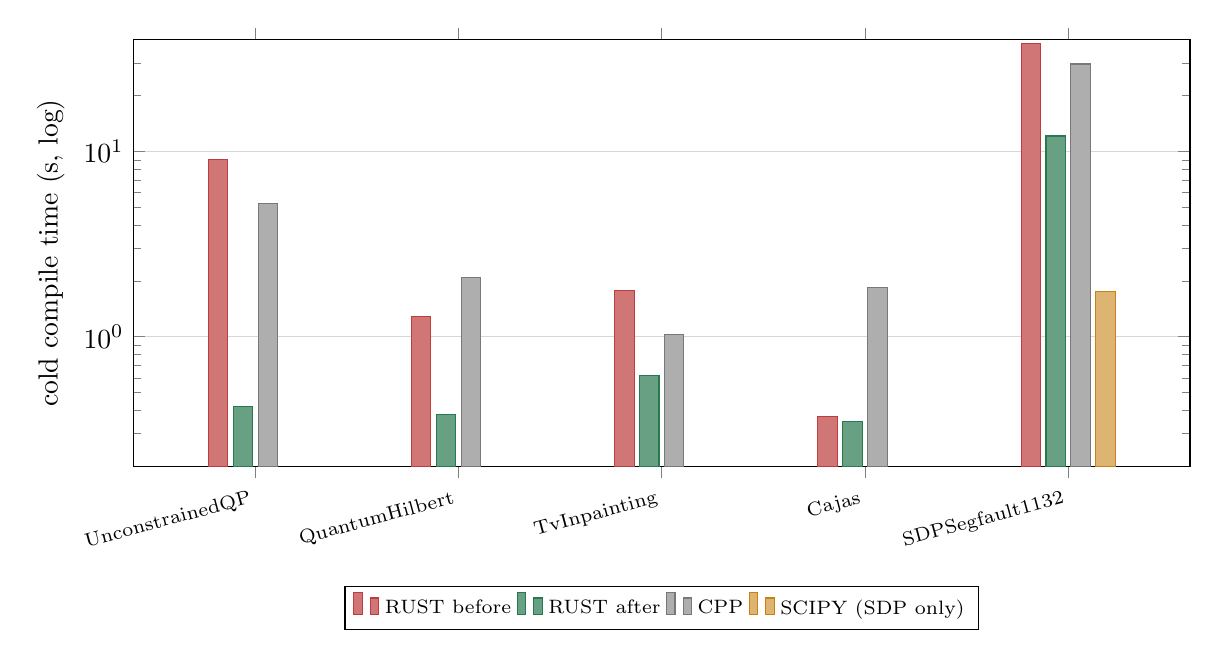
\begin{tikzpicture}
\begin{axis}[
  ybar, width=15cm, height=7cm, bar width=7pt,
  ymode=log, log origin=infty, ymin=0.2, ymax=40,
  ylabel={cold compile time (s, log)},
  symbolic x coords={UnconstrainedQP, QuantumHilbert, TvInpainting, Cajas, SDPSegfault1132},
  xtick=data, x tick label style={font=\scriptsize, rotate=15, anchor=north east},
  legend style={font=\scriptsize, at={(0.5,-0.28)}, anchor=north, legend columns=4},
  ymajorgrids, grid style={grey!30}, enlarge x limits=0.15,
]
\addplot[fill=oldc!70, draw=oldc] coordinates {(UnconstrainedQP,9.04) (QuantumHilbert,1.29) (TvInpainting,1.77) (Cajas,0.37) (SDPSegfault1132,38)};
\addplot[fill=newc!70, draw=newc] coordinates {(UnconstrainedQP,0.42) (QuantumHilbert,0.38) (TvInpainting,0.62) (Cajas,0.35) (SDPSegfault1132,12.1)};
\addplot[fill=grey!60, draw=grey] coordinates {(UnconstrainedQP,5.24) (QuantumHilbert,2.08) (TvInpainting,1.03) (Cajas,1.85) (SDPSegfault1132,29.6)};
\addplot[fill=constc!60, draw=constc] coordinates {(SDPSegfault1132,1.75)};
\legend{RUST before, RUST after, CPP, SCIPY (SDP only)}
\end{axis}
\end{tikzpicture}
\caption{Before/after on the five classes (log scale). The ``before'' bar of SDPSegfault1132 is drawn
at the top of the axis: that run did not finish.}
\end{figure}

%======================================================================
\section{Step 0: a safe availability check}
\label{sec:step0}

\paragraph{Problem.} The default backend was chosen by \code{try: import cvxpy\_rust}. In a source
checkout without the compiled extension, that import \emph{succeeds}: the crate directory
\code{cvxpy\_rust/} at the repository root is importable as an empty namespace package. Settings then
selected RUST, and every solve died on a missing \code{build\_matrix\_serialized}. The same trap was hit
twice on the new machine with stale shared objects shadowing a fresh build.

\paragraph{Change (commit \code{56aa4e516}).} \code{settings.rust\_backend\_available()} imports the
module and checks for the entry-point attribute; the default, the explicit-RUST path (which now raises a
clear \code{ImportError}), and every test skip use it. Four tests stub \code{sys.modules} to cover the
namespace-package, missing-module and built-extension cases.

%======================================================================
\section{Step 1: three N-D correctness bugs}
\label{sec:step1}

The audit of 15 September found three RUST-only bugs, all on expressions with three or more axes.
Each is a misunderstanding of how an N-D array flattens in F-order, so we first fix the notation.

\subsection{F-order flattening of an N-D array}

For an array of shape $(s_0, s_1, \dots, s_{d-1})$ the flat F-order index of the multi-index
$(i_0, \dots, i_{d-1})$ is
\begin{equation}
  \label{eq:forder}
  \operatorname{flat}(i_0,\dots,i_{d-1}) \;=\; i_0 + s_0\big(i_1 + s_1(i_2 + \cdots)\big)
  \;=\; \sum_{a=0}^{d-1} i_a \prod_{b<a} s_b .
\end{equation}
The \emph{first} axis varies fastest. For a batch of matrices of shape $(B, n, n)$ this means the
batch index is the fastest axis and entry $(\beta, i, j)$ sits at $\beta + B(i + nj)$.

\begin{figure}[H]
\centering
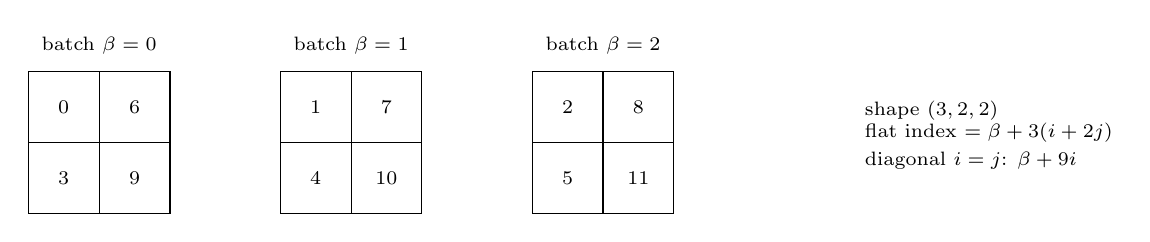
\begin{tikzpicture}[every node/.style={font=\scriptsize}]
  \foreach \b in {0,1,2} {
    \begin{scope}[shift={(3.2*\b,0)}]
      \node[anchor=south] at (0.9,1.9) {batch $\beta=\b$};
      \foreach \i in {0,1} \foreach \j in {0,1} {
        \pgfmathtruncatemacro{\flat}{\b + 3*(\i + 2*\j)}
        \draw (0.9*\j,1.8-0.9*\i-0.9) rectangle ++(0.9,0.9);
        \node at (0.9*\j+0.45,1.8-0.9*\i-0.45) {$\flat$};
      }
    \end{scope}
  }
  \node[align=left] at (12.2,1.0) {shape $(3,2,2)$\\ flat index $=\beta + 3(i+2j)$\\[2pt] diagonal $i=j$: $\beta + 9i$};
\end{tikzpicture}
\caption{F-order flat indices of a $(3,2,2)$ array. The three diagonals are $\{0,9\},\{1,10\},\{2,11\}$:
row $\beta + 9i$ for $i=0,1$.}
\label{fig:forder}
\end{figure}

\subsection{Bug 1: 3-D sparse constants}

The serializer converted every sparse constant to CSC before packing it. SciPy's CSC is 2-D only, so a
batched sparse constant (the $(2,2,2)$ mask that \code{lambda\_max} on a batch builds) raised
\emph{``CSC format must be 2D''}. A constant leaf's tensor, however, is simply the F-order flattening of
its value placed in the constant column: entry with multi-index $\mathbf{i}$ goes to row
$\operatorname{flat}(\mathbf{i})$. The fix computes those flat rows with
\code{np.ravel\_multi\_index(coo.coords, shape, order="F")} and emits the constant as a single CSC
column of length $\prod s_a$. Nothing on the Rust side changed: it already read a sparse leaf column by
column and pushed row $jm+i$, which for a one-column matrix is just $i$.

\subsection{Bug 2: N-D \code{vstack} row order}

\code{vstack} promotes each argument to at least 2-D and concatenates along axis 0. The Rust
implementation first concatenated the arguments' flattened tensors (``hstack'') and then permuted rows,
but the permutation was only computed for 2-D output; for 3-D and 4-D output it fell into a branch that
concatenated flat buffers, which is the wrong order. The correct permutation has one clean statement.
Let the output have shape $(R, s_1, \dots, s_{d-1})$ and let $t$ index the trailing dimensions,
$t \in \{0,\dots,\tau-1\}$ with $\tau = \prod_{a\ge1} s_a$. Argument $a$ contributes $\rho_a = |\text{arg}_a|/\tau$
leading rows and its own flat index of (leading row $r$, trailing $t$) is $r + \rho_a t$ by
\eqref{eq:forder}. Iterating the output in F-order therefore visits, for each $t$, each argument in
turn, each of its $\rho_a$ rows:
\begin{equation}
  \label{eq:vstack}
  \text{order} = \big[\ \text{offset}_a + r + \rho_a t \ :\ t = 0..\tau{-}1,\ a = 0..A{-}1,\ r = 0..\rho_a{-}1\ \big].
\end{equation}
This is exactly what \code{np.vstack(...).flatten(order="F")} produces on index arrays, covers
1-D arguments ($\rho_a=1$) and 2-D arguments alike, and replaced the special-cased code.

\begin{figure}[H]
\centering
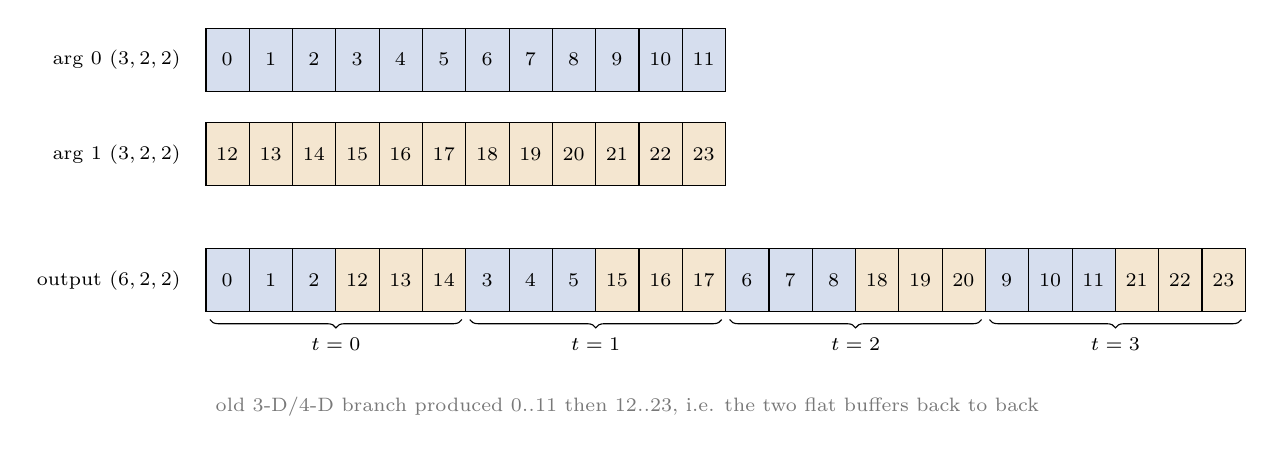
\begin{tikzpicture}[every node/.style={font=\scriptsize}]
  \node[anchor=east] at (-0.2,1.2) {arg 0 $(3,2,2)$};
  \foreach \k in {0,...,11} { \draw[fill=varc!20] (0.55*\k,0.8) rectangle ++(0.55,0.8); \node at (0.55*\k+0.27,1.2) {\k}; }
  \node[anchor=east] at (-0.2,0.0) {arg 1 $(3,2,2)$};
  \foreach \k in {0,...,11} { \pgfmathtruncatemacro{\v}{\k+12} \draw[fill=constc!20] (0.55*\k,-0.4) rectangle ++(0.55,0.8); \node at (0.55*\k+0.27,0.0) {\v}; }
  \node[anchor=east] at (-0.2,-1.6) {output $(6,2,2)$};
  \foreach \k in {0,...,23} {
    \pgfmathtruncatemacro{\t}{int(\k/6)} \pgfmathtruncatemacro{\w}{mod(\k,6)}
    \pgfmathtruncatemacro{\a}{int(\w/3)} \pgfmathtruncatemacro{\r}{mod(\w,3)}
    \pgfmathtruncatemacro{\v}{12*\a + \r + 3*\t}
    \ifnum\a=0 \draw[fill=varc!20] (0.55*\k,-2.0) rectangle ++(0.55,0.8); \else \draw[fill=constc!20] (0.55*\k,-2.0) rectangle ++(0.55,0.8); \fi
    \node at (0.55*\k+0.27,-1.6) {\v};
  }
  \foreach \t in {0,1,2,3} { \draw[decorate, decoration={brace, mirror, amplitude=3pt}] (3.3*\t+0.05,-2.1) -- (3.3*\t+3.25,-2.1) node[midway, below=3pt] {$t=\t$}; }
  \node[anchor=west, align=left, grey] at (0,-3.2) {old 3-D/4-D branch produced $0..11$ then $12..23$, i.e. the two flat buffers back to back};
\end{tikzpicture}
\caption{Row order for \code{vstack} of two $(3,2,2)$ arguments, equation \eqref{eq:vstack}: for each
trailing position $t$ (four of them), three rows of argument 0 then three of argument 1.}
\end{figure}

\subsection{Bug 3: batched \code{trace}}

\code{process\_trace} took $n$ from axis 0 and summed every entry whose row was a multiple of $n+1$
into output row 0. For a $(3,2,2)$ argument that treats a batch of three $2\times2$ matrices as one
$3\times3$ matrix. With figure~\ref{fig:forder}, the diagonal entry $(\beta,i,i)$ of a $(B,n,n)$
argument is at row $\beta + B\,i(n+1)$, so
\begin{equation}
  \text{row } r \text{ is diagonal} \iff \Big\lfloor \tfrac{r}{B} \Big\rfloor \bmod (n+1) = 0,
  \qquad \text{output row} = r \bmod B ,
\end{equation}
an $O(1)$ test per entry that reduces to the old one for $B=1$.

\subsection{Tests, and two bugs that are not Rust's}

Beyond SCIPY-vs-RUST unit cases for each operation, a cross-backend \emph{affine-map oracle} was
added to \code{test\_python\_backends.py}: for an expression $f$ of one variable and a point $x_0$,
\begin{equation}
  A\,\vecF(x_0) + b \;\overset{?}{=}\; \vecF\big(f(x_0)\big),
\end{equation}
with $f(x_0)$ evaluated numerically by CVXPY itself. Comparing backends with each other cannot catch a
bug they all share; this can, and it did: N-D \code{hstack} and \code{concatenate(axis=None)}
canonicalize in flat F-order on \emph{every} backend while their numeric value follows NumPy, and COO
fails on N-D sparse constants. Those cases are marked \code{xfail} and an upstream issue is drafted
(\code{rust\_benchmarks/UPSTREAM\_ISSUE\_ND\_STACK\_DRAFT.md}).

%======================================================================
\section{Step 2: one accumulating kernel for \code{mul} and \code{rmul}}
\label{sec:kernel}

This is the change that removed most of the time (commit \code{febfd64fc}).

\subsection{The two block-diagonal products}

Let the argument tensor $T$ represent $\vecF(X)$ for a matrix-shaped expression $X$ with $k$ rows.
The two constant multiplications CVXPY emits are
\begin{align}
  \text{\code{mul}:}\quad & \vecF(AX) = (I_k \otimes A)\,\vecF(X), & A \in \R^{a_r \times a_c}, \label{eq:mul}\\
  \text{\code{rmul}:}\quad & \vecF(XA) = (A^\T \otimes I_k)\,\vecF(X), & A \in \R^{n \times p}. \label{eq:rmul}
\end{align}
Both are block-structured. In \eqref{eq:mul} the input row $\rho$ of $T$ splits as
$\rho = \beta a_c + l$ (block $\beta$, column $l$ of $A$) and the output row is $\beta a_r + o$; column
$l$ of $A$ is what one unit of input part $l$ contributes to the block's $a_r$ outputs. In
\eqref{eq:rmul} the input row splits as $\rho = l\,k + i$ (row $i$ of $X$, column $l$ of $X$ = row $l$ of
$A$), the output row is $j\,k + i$, and row $l$ of $A$ is what one unit of $X_{il}$ contributes to the $p$
outputs of row $i$. In both cases:
\begin{quote}
\emph{an output entry (bucket, position, tensor column, parameter slice) is the sum, over the
contribution index $l$, of $M_{o,l} \cdot T_{(\text{bucket},l),\,\text{col},\,\text{param}}$},
\end{quote}
with $M = A$ for \code{mul} and $M = A^\T$ for \code{rmul}. Two products can only land on the same
output entry if they share the bucket, the tensor column and the parameter slice.

\subsection{What the old kernels did}

Six kernels (dense column-major, dense row-major, sparse CSC; each for left and right) implemented
\eqref{eq:mul}--\eqref{eq:rmul} the same way: for every entry $e$ of $T$, for every nonzero $M_{o,l}$ in
the contribution column, push a new COO entry. Nothing merged anything. The number of pushes is
\begin{equation}
  \label{eq:pushes}
  P_{\text{old}} = \sum_{e \in T} \nnz\big(M_{:,\,l(e)}\big),
\end{equation}
each push writes 32 bytes, and the entire result is later sorted (section~\ref{sec:assembly}) and
summed by SciPy. The pre-allocation was $\nnz(T)\cdot a_r$ entries.

For UnconstrainedQP the expression is $H^{\mathsf H}\,\mathrm{Err}\,H\,x$ with $H$ a dense
$252\times252$ DFT matrix; the tensor entering the dense \code{rmul} has $2.3$M entries, so
$P_{\text{old}} \approx 2.3\text{M} \times 252 \approx 5.8\times10^8$ pushes, about 18\,GB of
writes and a $5.8\times10^8$-element sort. For SDPSegfault1132 the \code{rmul} by $V^\T$ (dense
$100\times99$) on $V G$ produced $\sim 10^8$ entries of which the following \code{diag} keeps 1\%;
the pre-allocation alone was several GB and the baseline run died.

\subsection{The new kernel: group, accumulate, emit}

\code{multiply\_grouped} replaces all six kernels with the following (figure~\ref{fig:grouped}).

\begin{algorithmic}[1]
\Require contribution matrix $M$ ($n_{\text{out}} \times n_{\text{in}}$, dense column-major or CSC), tensor $T$, side (left/right), optional wanted output rows $W$
\State counting-sort the entry indices of $T$ by bucket \Comment{$O(\nnz(T) + \#\text{buckets})$}
\State $\text{acc} \gets 0^{\,n_{\text{out}}}$ \Comment{one dense workspace, reused}
\For{each bucket $\beta$ with entries (and, if $W$ given, with wanted rows)}
  \State sort the bucket's entry indices by (col, param) \Comment{colliding entries become adjacent}
  \For{each maximal run $G$ with equal (col, param)}
    \For{each entry $e \in G$ with part $l(e)$ and value $v_e$}
      \State $\text{acc}[o] \mathrel{+}= M_{o,l(e)}\, v_e$ for the nonzeros $o$ of column $l(e)$ (or only $o \in W_\beta$)
    \EndFor
    \State emit $(\text{out\_row}(\beta,o),\ \text{col},\ \text{param},\ \text{acc}[o])$ for every touched $o$ with $\text{acc}[o] \ne 0$; reset those cells
  \EndFor
\EndFor
\end{algorithmic}

\begin{figure}[H]
\centering
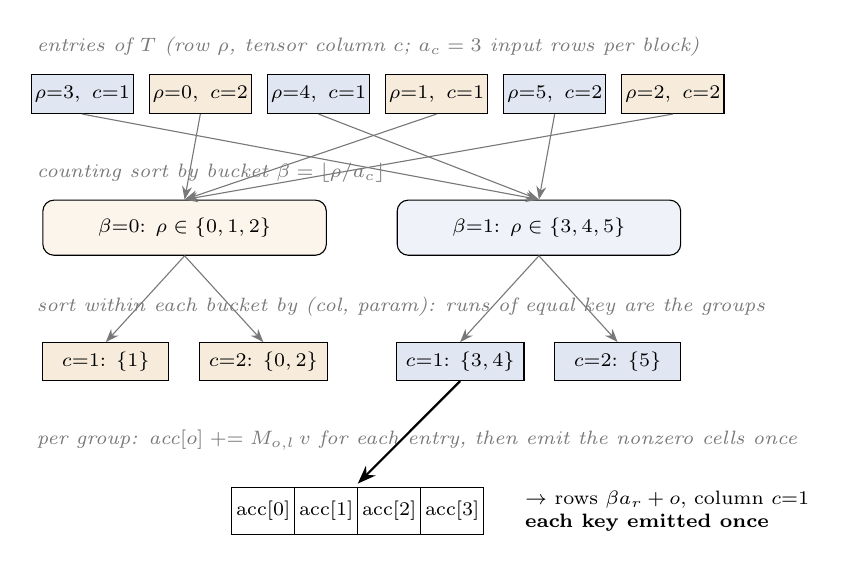
\begin{tikzpicture}[every node/.style={font=\scriptsize},
  ent/.style={draw, minimum width=13mm, minimum height=5mm, inner sep=1pt},
  lbl/.style={font=\scriptsize\itshape, grey, anchor=west}]
  \node[lbl] at (0,3.0) {entries of $T$ (row $\rho$, tensor column $c$; $a_c = 3$ input rows per block)};
  \foreach \i/\r/\c/\col in {0/3/1/varc, 1/0/2/constc, 2/4/1/varc, 3/1/1/constc, 4/5/2/varc, 5/2/2/constc} {
    \node[ent, fill=\col!15] (e\i) at (1.5*\i+0.7,2.4) {$\rho{=}\r,\ c{=}\c$};
  }
  \node[lbl] at (0,1.4) {counting sort by bucket $\beta = \lfloor \rho / a_c \rfloor$};
  \node[draw, rounded corners, fill=constc!8, minimum width=3.6cm, minimum height=7mm] (b0) at (2.0,0.7) {$\beta{=}0$: $\rho\in\{0,1,2\}$};
  \node[draw, rounded corners, fill=varc!8, minimum width=3.6cm, minimum height=7mm] (b1) at (6.5,0.7) {$\beta{=}1$: $\rho\in\{3,4,5\}$};
  \foreach \i in {1,3,5} \draw[-{Stealth}, grey] (e\i.south) -- (b0.north);
  \foreach \i in {0,2,4} \draw[-{Stealth}, grey] (e\i.south) -- (b1.north);
  \node[lbl] at (0,-0.3) {sort within each bucket by (col, param): runs of equal key are the groups};
  \node[draw, fill=constc!15, minimum width=1.6cm] (g0a) at (1.0,-1.0) {$c{=}1$: $\{1\}$};
  \node[draw, fill=constc!15, minimum width=1.6cm] (g0b) at (3.0,-1.0) {$c{=}2$: $\{0,2\}$};
  \node[draw, fill=varc!15, minimum width=1.6cm] (g1a) at (5.5,-1.0) {$c{=}1$: $\{3,4\}$};
  \node[draw, fill=varc!15, minimum width=1.6cm] (g1b) at (7.5,-1.0) {$c{=}2$: $\{5\}$};
  \draw[-{Stealth}, grey] (b0.south) -- (g0a.north); \draw[-{Stealth}, grey] (b0.south) -- (g0b.north);
  \draw[-{Stealth}, grey] (b1.south) -- (g1a.north); \draw[-{Stealth}, grey] (b1.south) -- (g1b.north);
  \node[lbl] at (0,-2.0) {per group: $\text{acc}[o] \mathrel{+}= M_{o,l}\, v$ for each entry, then emit the nonzero cells once};
  \foreach \o in {0,1,2,3} { \draw (2.6+0.8*\o,-3.2) rectangle ++(0.8,0.6); \node at (3.0+0.8*\o,-2.9) {acc[\o]}; }
  \draw[-{Stealth}, thick] (g1a.south) -- (4.2,-2.55);
  \node[anchor=west, align=left] at (6.2,-2.9) {$\to$ rows $\beta a_r + o$, column $c{=}1$\\ \textbf{each key emitted once}};
\end{tikzpicture}
\caption{The grouped kernel. Only entries in the same bucket, column and parameter slice can collide,
so after two sorts every collision is a run of adjacent entries, and each run is resolved in a dense
workspace of one block's size.}
\label{fig:grouped}
\end{figure}

\subsection{Why it is faster, and why it is the same arithmetic}

The multiply-add count does not change: $P_{\text{new}} = P_{\text{old}}$ in the dense case.
What changes is what each product costs and what is left afterwards:
\begin{center}
\footnotesize
\setlength{\tabcolsep}{4pt}
\begin{tabular}{lll}
\toprule
 & old (push per product) & new (accumulate per group) \\
\midrule
per product & 32-byte push to a growing vector & one FMA into an $L1$-resident workspace \\
output entries & $P$ (with duplicates) & $\#\{$unique (row, col, param)$\}$ \\
memory & $32P$ bytes, pre-allocated up front & $32 \cdot \nnz(\text{output})$ \\
downstream sort & over $P$ entries & over unique entries \\
extra cost & --- & counting sort $O(\nnz T)$; per-bucket sort $O(b \log b)$ \\
\bottomrule
\end{tabular}
\end{center}
For \code{rmul} the contribution matrix is $A^\T$; its column $l$ is row $l$ of $A$, which is
\emph{contiguous} in row-major storage. Dense row-major data is therefore used as-is, dense column-major
data is transposed once ($O(np)$), and CSC data is converted to CSR once ($O(\nnz A)$): the old sparse
\code{rmul} scanned every CSC column for every entry, $O(\nnz(T)\cdot\nnz(A))$, which the audit had
flagged on QuantumHilbertMatrix (\code{AxI} is $512\times512$ with 9\,520 nonzeros).

The randomized tests (\code{grouped\_kernel\_tests}) build random $A$ (about half zeros), random
tensors with deliberately repeated keys and three parameter slices, and check the kernel against the
per-product reference \eqref{eq:pushes} summed by key, for all six original variants and for restricted
row sets.

\subsection{Effect}

\begin{center}
\begin{tabular}{lrrr}
\toprule
class & RUST before & RUST after step 2 & CPP \\
\midrule
UnconstrainedQP & 9.04 s & 0.45 s & 5.24 s \\
QuantumHilbertMatrix & 1.29 s & 0.40 s & 2.08 s \\
TvInpainting & 1.77 s & 1.53 s & 1.03 s \\
Cajas & 0.37 s & 0.35 s & 1.85 s \\
SDPSegfault1132 & crashed & 15.4 s & 29.6 s \\
\bottomrule
\end{tabular}
\end{center}
The eight \code{process\_mul} calls in UnconstrainedQP fell from about 4.2\,s to 0.2\,ms each; the
cross-backend gate (\code{verify\_backends.py}, 18 ASV cases $\times$ 3 backends against SCIPY) reports
every stuffed matrix identical.

%======================================================================
\section{Step 3: row selection, assembly and elementwise multiply}
\label{sec:assembly}

With the kernels fixed, a per-node profiler (\code{CVXPY\_RUST\_PROFILE=1}, added in this step because
\code{perf} is blocked on the machine) showed where the next seconds were.

\subsection{Row selection by a dense map (TvInpainting)}

TvInpainting's total variation stacks the horizontal and vertical differences of three
$512\times512$ images: a \code{vstack} of six rows of width $261\,121$, i.e. the permutation
\eqref{eq:vstack} with $\rho_a=1$ and $\tau = 261\,121$. That permutation is a stride-6 interleave,
so none of \code{select\_rows}'s fast paths (identity, contiguous offset, reversal) apply and it fell
to the general path, which built a \code{HashMap<old\_row, Vec<new\_row>>} with 1.57\,M keys. The
profiler attributed 1.09\,s of a 1.24\,s build to that one node.

A permutation, or any row map $\pi$ from old rows to (possibly several) new rows, is a sparse relation
on $\{0,\dots,m_{\text{old}}-1\}$, and the natural structure for it is a CSR-style table: count new
rows per old row, prefix-sum, scatter. Building it is $O(m_{\text{old}} + |\pi|)$ with no hashing,
and lookups are two array reads. The \code{vstack} node fell from 1\,086\,ms to 229\,ms and the class
from 1.53\,s to 0.62\,s.

\subsection{Assembly: direct sort and coalescing}

The final assembly (figure~\ref{fig:pipeline}) computes the flat row $jm+i$ of every entry and sorts,
because SciPy's COO$\to$CSC constructor degrades to linear passes on row-sorted input. It sorted an
index array by an indirect key (\code{order.sort\_by\_key(|i| rows[i])}), which is cache-hostile at
$10^8$ entries. It now sorts 16-byte records $(\text{flat row},\ \text{param},\ \text{index})$ directly
and, in the same pass, sums adjacent duplicates, so Python never receives the duplicates that a sum of
overlapping affine terms produces. On SDPSegfault1132 that is 148.5\,M entries in, 49.5\,M out; the
already-sorted fast path was tightened to ``sorted and unique''.

\subsection{Elementwise multiply}

\code{mul\_elem} grouped its data entries by row in a \code{Vec<Vec<(f64,i64)>>} (one heap
allocation per row) and looped over that per argument entry. It now uses the same flat CSR-style table
and, when no row has more than one data entry (every dense or sparse constant, and every parameter),
a dense lookup with no inner loop. On the 148\,M-entry \code{mul\_elem} of SDP this took 2.3\,s to
2.1\,s; the cost that remains is the memory traffic of the pushes themselves.

%======================================================================
\section{Step 4a: lowering shared subexpressions once (DAG memo)}
\label{sec:memo}

CVXPY expression graphs are DAGs: an expression object used in several constraints, or several times
in one, is one LinOp with several parents. The serializer walked the graph as a tree, so a shared node
was re-emitted and re-lowered at every use. The July measurements found tree-nodes/unique-LinOps ratios
of 3.6 on QuantumHilbertMatrix and 2.1 on UnconstrainedQP.

\paragraph{Change (commit \code{41e40c22d}).} A pre-pass over the trees counts, per LinOp object,
how many \code{args} edges reach it. A node reached at least twice is emitted at its first occurrence
wrapped in a \code{def} marker with an id, and as a \code{ref} node (carrying only its shape and the
id) afterwards. The Rust deserializer moves each defined subtree into a shared table and leaves a
\code{Ref} in the tree. Lowering a \code{Ref} evaluates the shared subtree once into a
\code{OnceLock} (so it is safe when constraints are lowered in parallel by rayon) and clones the tensor
per use. Leaves and constant \emph{data} subtrees are never memoized, so the const-times-variable fast
path and the constant extraction still see plain nodes.

\begin{figure}[H]
\centering
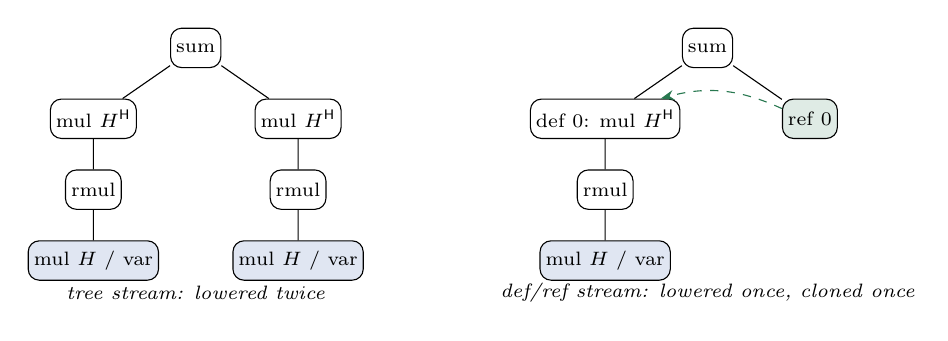
\begin{tikzpicture}[every node/.style={font=\scriptsize, draw, rounded corners, inner sep=2pt, minimum height=5mm}, level distance=9mm, sibling distance=26mm, >={Stealth}]
  \begin{scope}
    \node (s) {sum}
      child { node {mul $H^{\mathsf H}$} child { node {rmul} child { node[fill=varc!15] {mul $H$ / var} } } }
      child { node {mul $H^{\mathsf H}$} child { node {rmul} child { node[fill=varc!15] {mul $H$ / var} } } };
    \node[draw=none, below=26mm of s, font=\scriptsize\itshape] {tree stream: lowered twice};
  \end{scope}
  \begin{scope}[shift={(6.5,0)}]
    \node (s2) {sum}
      child { node (d) {def 0: mul $H^{\mathsf H}$} child { node {rmul} child { node[fill=varc!15] {mul $H$ / var} } } }
      child { node[fill=newc!15] (r) {ref 0} };
    \draw[->, dashed, newc] (r) to[bend right=20] (d);
    \node[draw=none, below=26mm of s2, font=\scriptsize\itshape] {def/ref stream: lowered once, cloned once};
  \end{scope}
\end{tikzpicture}
\caption{The two $H^{\mathsf H}\,\mathrm{Err}\,H$ sums of UnconstrainedQP as the serializer saw them
before (left) and after (right) the DAG memo.}
\end{figure}

The effect is bounded by how much the model reuses objects: QuantumHilbertMatrix improved from
0.40\,s to 0.36\,s; SDPSegfault1132 did not move at all because its three occurrences of
$VGV^\T$ are three distinct Python objects.

%======================================================================
\section{Step 4b: pushing row selection down through the tree}
\label{sec:pushdown}

\subsection{The structural loss}

SDPSegfault1132 (issue \#1132) has $G \in \mathbb{S}^{99}$ PSD (4\,950 free entries),
$V \in \R^{100\times99}$ dense, and forms
\begin{equation}
  \label{eq:sdp}
  A = \mathbf{1}\otimes \operatorname{diag}(VGV^\T)^\T,\quad
  B = \operatorname{diag}(VGV^\T)\otimes \mathbf{1}^\T,\quad
  C = \big\| W \circ (A + B - 2VGV^\T - D) \big\|_F .
\end{equation}
$VGV^\T$ is a dense $100\times100$ matrix every entry of which depends on all of $G$: its Jacobian
is $10\,000 \times 4\,950$ dense, $49.5$\,M nonzeros. \code{diag} then keeps 100 rows of the
10\,000. Lowering the argument in full and then filtering costs the full product, and the profiler
showed each \code{diag\_mat} node at 755\,ms inclusive.

\subsection{Restricted lowering}

Define, for a node $f$ and a set $R$ of its output rows, the \emph{restricted lowering}
$\mathcal{L}_R(f)$: the tensor of $f$ with only the rows in $R$ populated. The full lowering is
$\mathcal{L}(f) = \mathcal{L}_{\text{all}}(f)$, and trivially
$\mathcal{L}_R(f) = \Pi_R\,\mathcal{L}(f)$ for the row filter $\Pi_R$. The point is that for most
operations $\mathcal{L}_R(f)$ can be computed from a restricted lowering of the children, with a
set $R'$ that is much smaller than ``all'':
\begin{center}
\footnotesize
\setlength{\tabcolsep}{4pt}
\begin{tabular}{lll}
\toprule
node $f$ & rows of the child needed for $R$ & then \\
\midrule
neg, reshape, mul\_elem, div & $R' = R$ & apply the node's own map \\
sum & $R' = R$ for every child & concatenate \\
index, transpose (row map $\pi$) & $R' = \pi(R)$ & \code{select\_rows}$(\pi)$, filter to $R$ \\
diag\_mat (step $s$, offset $c$) & $R' = \{\, r s + c : r \in R \,\}$ & diagonal map \\
trace ($B$ batches of $n\times n$) & $R' = \{\, \beta + B\,i(n{+}1) : \beta \in R,\ i<n \,\}$ & diagonal sum \\
mul $=(I_k\otimes A)$ & whole blocks: $\beta = \lfloor r/a_r \rfloor$, $R' = \bigcup_\beta [\beta a_c, (\beta{+}1)a_c)$ & kernel with $W=R$ \\
rmul $=(A^\T\otimes I_k)$ & whole rows of $X$: $i = r \bmod k$, $R' = \{ i + k\,l : l < n \}$ & kernel with $W=R$ \\
anything else & all & lower fully, filter to $R$ \\
\bottomrule
\end{tabular}
\end{center}
The restriction is only used when the consumer reads at most half of the child's rows; otherwise the
child is lowered in full. Because the kernel of section~\ref{sec:kernel} accepts the wanted rows
$W$, a restricted \code{rmul} does \emph{not} compute every output column of a needed row of $X$ and
throw most away: buckets without wanted rows are skipped before their sort, and the dense
accumulation touches only the wanted positions. For $\operatorname{diag}(VGV^\T)$ that turns the
per-group work from $99$ (all output columns of row $i$) into $1$ (column $i$).

\begin{figure}[H]
\centering
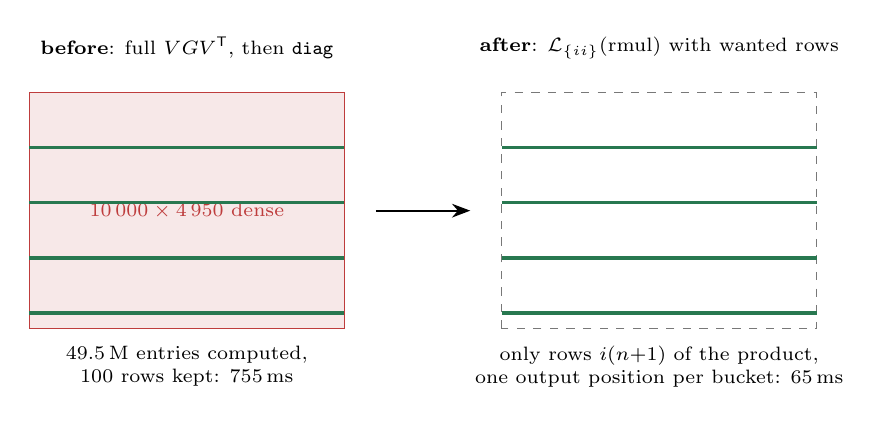
\begin{tikzpicture}[every node/.style={font=\scriptsize}]
  % full
  \node[anchor=south] at (2.0,3.3) {\textbf{before}: full $VGV^\T$, then \code{diag}};
  \draw[fill=oldc!12, draw=oldc] (0,0) rectangle (4,3);
  \node[oldc] at (2,1.5) {$10\,000 \times 4\,950$ dense};
  \foreach \i in {0.2,0.9,1.6,2.3} { \draw[very thick, newc] (0,\i) -- (4,\i); }
  \node[anchor=north, align=center] at (2,-0.1) {49.5\,M entries computed,\\ 100 rows kept: 755\,ms};
  % restricted
  \node[anchor=south] at (8.0,3.3) {\textbf{after}: $\mathcal{L}_{\{ii\}}(\text{rmul})$ with wanted rows};
  \draw[draw=grey, dashed] (6,0) rectangle (10,3);
  \foreach \i in {0.2,0.9,1.6,2.3} { \draw[very thick, newc] (6,\i) -- (10,\i); }
  \node[anchor=north, align=center] at (8,-0.1) {only rows $i(n{+}1)$ of the product,\\ one output position per bucket: 65\,ms};
  \draw[-{Stealth}, thick] (4.4,1.5) -- (5.6,1.5);
\end{tikzpicture}
\caption{Row push-down on $\operatorname{diag}(VGV^\T)$. The rows the consumer reads are known
before the product is formed, so the product is formed only for them.}
\end{figure}

The tests in \code{partial.rs} lower \code{diag}, \code{index}, \code{trace}, \code{mul\_elem} and
\code{div} over dense matmul chains (with a transpose, a negation and a sum in between) both fully
and restricted, and assert $\mathcal{L}_R(f) = \Pi_R \mathcal{L}(f)$ entry by entry.

\subsection{Effect and what is left on SDP}

Each \code{diag\_mat} fell from 755\,ms to 65\,ms and the class from 13.6\,s to 12.1\,s. The
profile of the remaining build (13.9\,s total including Python) is now honest about the problem:
\begin{center}
\begin{tabular}{lrl}
\toprule
node & inclusive & note \\
\midrule
\code{mul\_elem} ($W\circ\cdot$) & 5.45 s & 148.5\,M raw entries in and out \\
\quad of which \code{sum} of 4 terms & 3.34 s & $A$, $B$, $-2VGV^\T$, $D$: $3\times49.5$\,M copied \\
\quad\quad of which two \code{kron\_r} & 2.7 s & each replicates 100 diagonal rows 100 times \\
assembly (sort + coalesce) & 3.32 s & $148.5$\,M $\to$ $49.5$\,M unique \\
\bottomrule
\end{tabular}
\end{center}
The stuffed matrix of this problem genuinely has $49.5$\,M nonzeros; SciPy reaches it in 1.75\,s
because its intermediates are CSC matrices that are coalesced at every operation, so the three
overlapping terms are merged by a sparse addition rather than concatenated and sorted. In the COO
design, coalescing inside large \code{sum} nodes (sort and merge before the elementwise multiply and
the assembly) would remove roughly 2\,s; going further needs a different intermediate representation.

%======================================================================
\section{Per-problem attribution}

\begin{table}[H]
\centering
\footnotesize
\setlength{\tabcolsep}{5pt}
\begin{tabular}{lrrrrrr}
\toprule
class & baseline & 2: kernel & 3: select/asm & 4a: memo & 4b: push-down & CPP \\
\midrule
UnconstrainedQP & 9.04 & 0.45 & 0.40 & 0.40 & 0.42 & 5.24 \\
QuantumHilbertMatrix & 1.29 & 0.40 & 0.40 & 0.36 & 0.38 & 2.08 \\
TvInpainting & 1.77 & 1.53 & 0.62 & 0.62 & 0.62 & 1.03 \\
Cajas & 0.37 & 0.35 & 0.35 & 0.35 & 0.35 & 1.85 \\
SDPSegfault1132 & --- & 15.4 & 13.6 & 13.6 & 12.1 & 29.6 \\
\bottomrule
\end{tabular}
\caption{Cold compile time (s) after each step. Differences of $\pm 0.05$\,s between columns are
run-to-run noise.}
\end{table}

\begin{description}
  \item[UnconstrainedQP] entirely the kernel: a dense $252\times252$ \code{rmul} on a 2.3\,M-entry
  tensor (complex, so the real canonicalization doubles everything) was $5.8\times10^8$ pushes and a
  sort of the same size. The DAG memo also lowers the two $H^{\mathsf H}\,\mathrm{Err}\,H$ terms
  once, but at 0.4\,s the class is now dominated by the Python side (canonicalization of the
  \code{kron} and complex reductions), not by \code{build\_matrix}.
  \item[QuantumHilbertMatrix] the kernel again, this time the sparse \code{rmul} by \code{AxI}
  ($512\times512$, 9\,520 nonzeros): the old code scanned every CSC column per entry
  ($O(\nnz T \cdot \nnz A)$); the CSR conversion makes it $O(\sum_e \nnz(A_{l(e),:}))$. The memo
  removed the repeated lowering of the partial-transpose subtree.
  \item[TvInpainting] the \code{vstack} permutation of six wide rows: HashMap $\to$ dense table.
  The assembly of its 3.9\,M entries takes 74\,ms; nothing else in the class exceeds 100\,ms.
  \item[Cajas] 803 constraints, each small: the parallel constraint path was already the fastest
  backend by $5\times$ and none of the changes touched what it does.
  \item[SDPSegfault1132] the kernel made it finish (no $\nnz(T)\cdot a_r$ pre-allocation, no
  $10^8$-entry sort per \code{rmul}); coalescing in assembly cut what Python receives by $3\times$;
  the push-down removed the two full products under \code{diag}. What remains is the dense Jacobian
  itself passing through \code{sum}, \code{mul\_elem} and the sort.
\end{description}

%======================================================================
\section{Validation}

Every commit was gated on the same evidence:
\begin{itemize}
  \item \code{cargo clippy -D warnings} (including \code{--tests}) and \code{cargo test}: 41 Rust
  unit tests, of which the randomized kernel tests, the restricted-vs-full push-down tests and the
  shared-subtree test are new.
  \item \code{test\_rust\_backend.py}, \code{test\_python\_backends.py},
  \code{test\_backend\_selection.py}: 378 passed, 7 expected failures (the upstream N-D
  \code{hstack}/\code{concatenate} and COO sparse-3-D cases).
  \item The broad suites with \code{CVXPY\_DEFAULT\_CANON\_BACKEND=RUST}
  (\code{test\_atoms}, \code{test\_problem}, \code{test\_dpp}, \code{test\_conic\_solvers},
  \code{test\_qp\_solvers}, \code{test\_complex}, \code{test\_constant\_atoms},
  \code{test\_canon\_methods}, \code{test\_expressions}, \code{test\_nd\_matmul},
  \code{test\_kron\_canon}): 1\,002 passed, 449 skipped for absent solvers, 0 failed.
  \item \code{verify\_backends.py}: the stuffed tensors of the 18 ASV backend cases identical
  (max $|\Delta| \le 8\times10^{-14}$) across RUST, CPP and COO against SCIPY, including all parameter
  slices.
\end{itemize}

%======================================================================
\section{Commits}

\begin{center}
\begin{tabular}{ll}
\toprule
commit & change \\
\midrule
\code{56aa4e516} & Require the built extension before defaulting to RUST \\
\code{f64ba8954} & Fix N-D sparse constants, N-D vstack row order, batched trace; affine-map oracle \\
\code{febfd64fc} & Accumulate mul/rmul per (block, column, parameter) group \\
\code{9205c076c} & Dense row-selection map; per-op profiling timer \\
\code{9bcd5447a} & Coalesce in assembly; flat row table for mul\_elem \\
\code{41e40c22d} & Lower shared LinOp subtrees once (DAG memo) \\
\code{7d2e1c3e5} & Push row selection down through mul/rmul and elementwise ops \\
\bottomrule
\end{tabular}
\end{center}
All are on \code{mellowyellow71/cvxrust:rust-backend-pr-20260915}; the documentation, tooling and
the upstream issue draft are on \code{rust-rebase-20260720}.

\end{document}
